%_____________________________________________________________________________________________ 
% LATEX Template: Department of Comp/IT BTech Project Reports
% Sample Chapter
% Sun Mar 27 10:25:35 IST 2011
%
% Note: Itemization, enumeration and other things not shown. A sample figure is included.
%_____________________________________________________________________________________________ 

\hypersetup{
    linkcolor=blue,
}
{\let\clearpage\relax \chapter{Literature Review}}
\section{Review Process}\\The systematic review was conducted by reading research papers. In order to retrieve the papers for our systematic review, we conducted keyword searches in Google Scholar, Scopus, Science Direct, ACM, ASCE and IEEE using the terms: 
\begin{enumerate}
    \item Road Route Alignment
    \item Route Planning System
    \item Route Selection System
\end{enumerate} By reading the titles of the research papers, The papers were downloaded. As a result of the search conducted on October 23, 2022, 180 research papers were downloaded based on their titles. A total of 35 papers were selected based on the inclusion and exclusion criteria for our systematic literature review. Papers involving the use of hyperspectral images, involving language other than english or performing route selection and alignment of road networks, pipelines, railway networks were excluded from our literature review. In reviewing the full texts of the remaining relevant papers, we collected the following types of information useful for a systematic literature review: Procedure of route alignment of roads and highways, different algorithms used for route selection and alignment including - Dijkstra, A star and other shortest path algorithms; Genetic algorithms, Swarm intelligence, Fuzzy logic and other DL/ML based algorithms; details of cost functions and factors involved in route selection considering economic, social and environmental implications, and analyzing the type and features of study area using various approaches and creating corresponding maps.
\begin{figure}[H]
	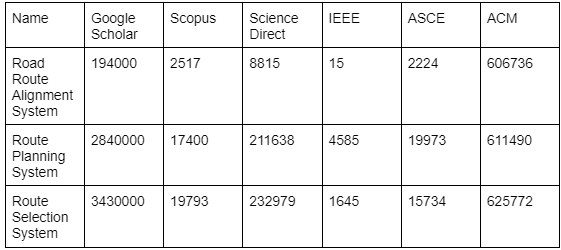
\includegraphics[width=475pt,height=275pt]{record.png}
	\caption{Total number of paper available for particular topic on particular site}
\end{figure}
\begin{figure}[H]
	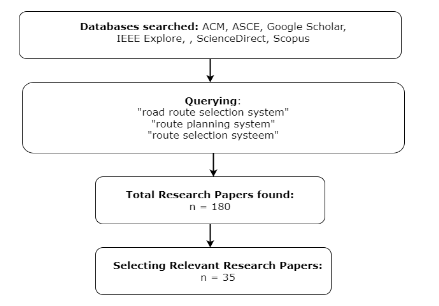
\includegraphics[width=475pt,height=325pt]{process.png}
	\caption{Process of Selection of papers for Systematic Literature Review using PRISMA analysis}
\end{figure}
\begin{figure}[H]
	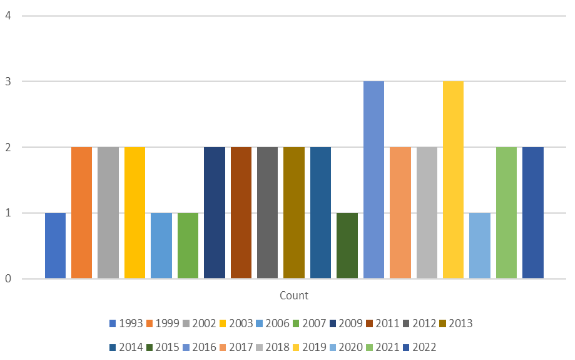
\includegraphics[width=475pt,height=275pt]{year_wise_count.png}
	\caption{Year wise count of included papers}
\end{figure}
\section{Stages involved in Route Alignment : }
\begin{figure}[H]
	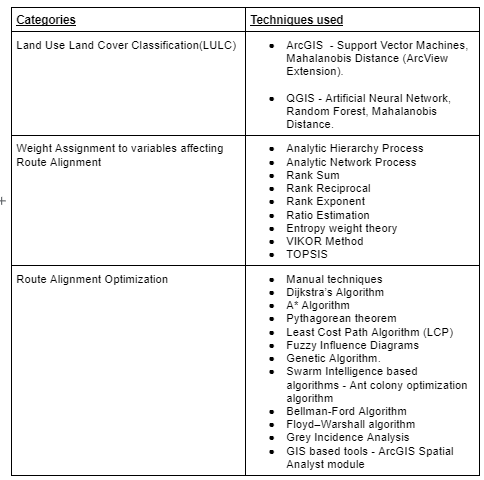
\includegraphics[width=475pt,height=425pt]{stages.png}
\end{figure}
\section{Literature Survey}
\subsection{Factors affecting route alignment : }
A correct plan for route alignment requires consideration of a number of factors or variables for construction of a function or model (\href{ https://ieeexplore.ieee.org/document/6675923}{Application of GIS in Highway Alignment with Soft Computing tools}). These factors include topography, environment, contour, geomorphology, geology, drainage, climate, cost, social, landuse and landcover.Topographic maps, aerial photographs, geological maps, soil maps, as well as various surveys can be used to analyze these factors. (\href{https://ieeexplore.ieee.org/document/8068706}{Remote Sensing and Geographical Information System Applications in Highway Alignment between the strips — Perundurai to Palani, Tamil Nadu, India}).Different types of factors can be measured via various cost functions , such as:
\begin{enumerate}
    \item Economic factors: can be calculated considering highway alignment and construction costs.
    \item Social and cultural factors: can be measured  considering accessibility cost, utility costs and proximity costs.
    \item  Environmental factors: can be estimated using Environmental Impact Assessment(EIA). It estimates the impact of route construction on the environment (soil, water, forests, climate) using penalty functions, and assigns corresponding values to alternative alignments.
\end{enumerate}

The variables are then represented in software like ArcGIS to create web maps and analyze geospatial data necessary for route alignment.The alignment plan is selected based on further studies performed with ArcGIS.
\subsection{Techniques for assigning weights to factors affecting route alignment : }
\textbf{Formal Decision Analysis : }
Formal decision analysis is used to assess the overall impact of different route alignments and decide the optimal alignments by ranking their impact on economic, social, environmental and utility factors. An initially used process from earlier times, it involved manually deciding the highway alignments, and then using decision analysis to rank them. (\href{https://ascelibrary.org/doi/10.1061/%28ASCE%290733-947X%281993%29119%3A3%28317%29 }{Decision Analysis of Alternative Highway Alignments}). Initially, the decision problem is structured by identifying the impact factors(land use, relocation, cultural & biological resources involved etc.), attributes to measure those impact factors, and selecting the alternative alignments possible by the stakeholders. Then, for every alignment, the attributes are assigned values depending on their impact  levels, and trade offs (considering penalty and cost functions).(\href{https://ascelibrary.org/doi/abs/10.1061/(ASCE)0733-947X(1999)125%3A2(144)}{GIS Platform for Multicriteria Evaluation of Route Alignments}). It is an effective process to evaluate alignments rationally and consider all multiple attributes involved in route alignment optimization but is time consuming due to manual intervention involved. Hence, further GIS tools including ArcGIS, Spatial Modules are developed to ease the process based on formal decision analysis techniques. Multi Criteria Evaluation or Multi Criteria Decision Analysis methods are also based on similar concepts, used to select important attributes or factors as per given area maps and purpose involved, which is then used to calculate the cost matrix for optimization. (\href{https://ascelibrary.org/doi/abs/10.1061/(ASCE)0733-947X(1999)125%3A2(144)}{GIS Platform for Multicriteria Evaluation of Route Alignments}). In this, various alternative attributes involved are ranked manually by the stakeholders, and the attributes are decided.(\href{https://link.springer.com/article/10.1007/s12517-017-3076-z
}{Multi-criteria GIS modeling for optimum route alignment planning in outer region of Allahabad City, India}). It is simple but less efficient, and can be optimized using different GIS tools for decision making.\\
\textbf{Weight ranking methods}
Multi-criteria weight methods are used to assign weights to input parameters/ factors affecting route alignment (as discussed in section 1). In each of the maps, the weight cost matrix is generated by weight assignment to the attributes and corresponding direction maps are plotted to visualize different factors involved in route alignment optimization. (\href{https://www.sciencedirect.com/science/article/pii/S1110982321000399}{Route alignment planning for a new highway between two cities using Geoinformatics techniques}). Five weight assignment methods are discussed as follows:
\begin{enumerate}
\item \textbf{Analytic Hierarchy Process (AHP) method - }
In this, a pairwise comparison matrix is constructed considering all input parameters. Each  attribute is given a score in the range of 10 by comparing the factors in terms of relative importance to an objective, and the resultant matrix generated is called the importance matrix. The importance matrix has the total weight of attributes, depicting its contribution towards best path identification.(Higher the weight, more important the factor).

\item \textbf{Rank Sum method - }
Rank sum is a non parametric procedure used in random sampling. 
Here, parameters involved are: 
wj is the normalized weight for the jth criteria
r is the rank position of the criterion
n is the total number of criteria under consideration

\item \textbf{Rank Reciprocal method - }
In this method, rank reciprocal weights are derived from the normalized reciprocals of a criterion’s rank.
Here, parameters involved are: 
wj is the normalized weight for the jth criteria
n is the total number of criteria under consideration 
r is the rank position of the criterion

\item \textbf{Rank Exponent method - }
In this, the decision makers initially assign weights to the most important factor/ criterion on a scale of 0-1, and then the weights of remaining factors are determined. 
Here,parameters involved are:
wj is the normalized weight for the jth criteria
r is the rank position of the criterion
n is the total number of criteria under consideration 

\item \textbf{ Ratio Estimation method - }
In this, an arbitrary weight is assigned to the most important factor on a scale of 0-100. The weights of remaining factors are estimated and smaller weights are assigned to less important factors. The procedure is continued until the weight to least important criterion is assigned. Finally, ratios of each of the factors are calculated with respect to least important factor, for relative comparison of factors involved.
\end{enumerate}
 \textbf{Entropy Weight Theory}
The concept of entropy weight theory is used to assign weights to different decision making variables involved in highway route alignment. Initially, an evaluation matrix of the route plan is created considering multiple attributes, objectives and indexes, and these are combined to generate a single synthesis index using entropy and entropy weight theory. Indexes can be classified as qualitative or quantitative, depending upon their impact and are assigned an index value using a 10 point system.Then the entropy weight decision making model is applied, which includes the following \textbf{4 steps:}
\begin{enumerate}
\item Scheme of evaluation, and indexes are decided, and a matrix is constructed considering cost and benefit of each scheme (or factor)
\item Entropy of each evaluation index is calculated as
Accordingly, the entropy weight of the index is calculated.
As per the entropy theory, a given index is a more important factor for decision making if it has smaller entropy weight and the difference of the same index for different schemes is larger.
\item Weight normalized matrix is constructed for each evaluation index, and the importance of factors are estimated using evaluation metrics such as - distance(difference between ideal point and evaluation point) and fidelity (distance of evaluation and ideal point / distance of ideal point to negative point).
\item Schemes (or factors) are selected according to their fidelity values. A scheme having smaller fidelity is considered more important for optimization. (\href{https://ascelibrary.org/doi/10.1061/41042%28349%2916}{Decision-Making Model of Highway Route Plan Based on Entropy and Entropy Weight Theory}).
\end{enumerate}
Towards the end, the best road alignment plan can be chosen by comparing synthesis index values. This decision making model is based on objective, hence the results are more realistic. Moreover, it also considers relationships between different factors involved in highway construction using their entropy, hence optimal routes can be selected.

\subsection{Techniques for Route alignment Optimization }
\textbf{Least Cost Path Algorithm (LCP)}\\Least Cost Path Algorithm is used to calculate least cost path joining start and end points for highway route alignment. With the help of the spatial analyst extension, ArcGIS software can generate the Least Cost Path Algorithm. Initially, a cost function is decided which considers the cost of construction (avoiding slopes, swampy areas), environmental area covered (water, forests etc.), social and cultural impact costs( damage to agricultural lands, moving of communities), via estimating multiple attributes involved using GIS based tools (\href{https://www.researchgate.net/publication/320005801_LEAST_COST_PATH_ALGORITHM_DESIGN_FOR_HIGHWAY_ROUTE_SELECTION}{Least Cost Path Algorithm Design for Highway Route Selection}). Once the cost parameters are decided, LCPA uses the cost-weighted distance and the direction surfaces for an area to determine a cost-effective route between a source and a destination location. The process is repeated until the source and destination points are connected via route having minimal cost. LCP analysis is used for optimizing social, environmental, economical, and technical aspects of the route alignment and can also be implemented effectively using GIS based tools as well (\href{https://link.springer.com/article/10.1007/s12517-017-3076-z}{ Multi-criteria GIS modeling for optimum route alignment planning in outer region of Allahabad City}).\\
\textbf{Fuzzy Logic}
Fuzzy logic refers to many-valued logic, in which the truth values of variables may be any real number between 0 and 1.A fuzzy logic approach can be useful when route alignment is being considered, since the results are not always accurate for any particular plan of route alignment.(\href{https://ieeexplore.ieee.org/document/6675923
}{Application of GIS in Highway Alignment with Soft Computing tools}). Fuzzy logic has also found applications in influence diagrams which can be used for constructing route alignment models. Using a fuzzy influence diagram, a model can be constructed to characterize the risk of a route alignment plan and to make a risk-based decision (\href{https://ieeexplore.ieee.org/document/6414422}{Research on Highway Alignment Decision-making based on complex system risk analysis}). It is advantage to use fuzzy logic when precise inputs are not required. \\
\textbf{Genetic algorithms and Swarm Intelligence}
Genetic algorithm is used for both constrained and unconstrained optimization that is inspired by natural selection, a process that drives biological evolution. GAs were first utilized for highway alignment optimization by Jong (1998). (\href{https://ascelibrary.org/doi/10.1061/40652%282003%297}{Optimizing Highway Networks- A Genetic Algorithms and Swarm Intelligence Based Approach})It uses the principle of orthogonal cutting planes,in which the straight line joining start and end points is divided into intervals(number of intervals decides the precision of optimization) (Diag. Pg 3), and each plane passes through an interval. It further states that the optimal highway alignment will always cross through exactly one point lying along each plane(formed passing through each interval of lines . 
There are \textbf{3 steps} involved in route optimization using Genetic algorithms : 
\begin{enumerate}
\item Genetic encoding and initial population is decided: For alignment of n intersection points in the intervals, the encoded solution has 2n genes. Hence, genes in chromosome and coordinates of intersection points are mapped ( as : (lambda)2i-1 = di … for all i = 1, 2, … n)
\item Genetic operators are applied to solved the optimization problem - it includes mutation based and crossover based operators - designed to work on the decoded intersection points
\item Optimal search is performed - Initially, the initial population is generated, and further generations, better solutions are searched by applying the genetic algorithm to minimize the objective function/ cost function. Cost function is decided considering the length dependent costs (construction, maintenance) and location dependent (right of way) costs. This step is used to produce optimized route alignments, to connect the start and end points by curve fitting.
\end{enumerate}
It takes longer time to search optimized route(s) using GAs, and the variation in cost functions reduce towards successive generations
GA can be further optimized by using swarm intelligence algorithm, which is inspired by the collective behavior of social insect colonies. It decides the evolution of genes in further generations, by selecting the intermediate planes for optimal search randomly. Hence, using SI with GA, reduces the computational efficiency and reaches optimal path quicker, although it is harder to apply SI for route optimization in regions with greater land variability, and route network optimization. (\href{https://www.sciencedirect.com/science/article/pii/S0968090X11001422}{Applicability of highway alignment optimization models}). To determine the optimum horizontal highway alignment using station points, an integrated GIS-GA model has also been developed.
\subsection{Other Techniques }
Hand drawn alignment sketches are also being used. In one study, hand-drawn alignment sketches on maps were easily converted into vector drawings, and all alignment coordinates and element data were stored in a data bank.Based on different criteria, the evaluation module for the generated vector representation of alignments is called a cost model (GMAPS-GCARS), which is actually formed by joining the nodes of a cost-model matrix, where each node is assigned a cost of traversing it - using the Dijkstra algorithm and Genetic Algorithm. Dijkstra's algorithm is commonly used for optimizing route alignments and finding shortest routes in many studies (\href{https://ascelibrary.org/doi/10.1061/40630%28255%29172 }{Interactive and Graphic Systems for Highway Location and Route Selection}).
\subsection{GIS tools for Route Alignment}
The alignment of routes has also been accomplished through the use of a variety of tools. ArcGIS, ArcInfo and ArcView are primarily used to digitize the land use, road networks and other variables within the given area. In these tools, initially the satellite images obtained are converted to vector layers. Then the layers are stacked onto each other, to obtain different cost criterion maps for land use/land cover, physical features, slope, forest, water areas, which are further converted to raster form and used to calculate cost matrix involved in alignment optimization. A Quantm computer-based planning tool was utilized for alignment optimization, which is capable of performing cost-based alignment optimization, generating low cost road or railway alignments automatically (\href{https://doi.org/10.1016/S0968-090X(00)00040-1}{New Technologies for Transport Route Selection}). As an alternative to a single least cost path, it provides a set of alternatives that take into consideration different social and economic factors and allow people to select their preferred alignment, resulting in lower costs. 
ArcGIS provides various tools for route alignment optimization, some of the tools used for route alignment include:
\begin{enumerate}
\item \textbf{Weighted Overlay Analysis (WOA) tool}: used for surface cost analysis to find out important factors involved in cost estimation using multi criteria evaluation/ multi attribute decision making. (\href{https://link.springer.com/article/10.1007/s12517-017-3076-z}{Multi-criteria GIS Modeling for Optimum Route Alignment Planning in Outer Region of Allahabad City}).
\item \textbf{Spatial Module}: used to perform alignment optimization by minimizing cost of path from source to destination.
\item \textbf{Polyline feature conversion tools}: used to convert optimum route alignment(s) calculated in raster form to polyline features for better visualization of path(s).
\end{enumerate}
GIS based tools can be utilized to perform overlays of maps, create buffers and rasters, analyze datasets of images through visualization, and cost optimization using various techniques.It provides a simple and efficient way to implement route alignment optimization through different modules available.



%_____________________________________________________________________________________________ 
